%Preâmbulo
\documentclass[12pt,a4paper]{article}
\usepackage[brazilian]{babel}
\usepackage[utf8]{inputenc}
\usepackage[left=2cm,right=2cm,top=2cm,bottom=2cm]{geometry}
\usepackage{amsmath,amsfonts,amssymb}
\usepackage{graphicx}
\graphicspath{{img/}}

\title{Inserir Tabela}
\author{César Antônio de Magalhães}
\date{\today}

%Corpo do texto
\begin{document}
	\begin{center}
		\begin{tabular}{cp{0.6\textwidth}}
			\begin{tabular}{c}
				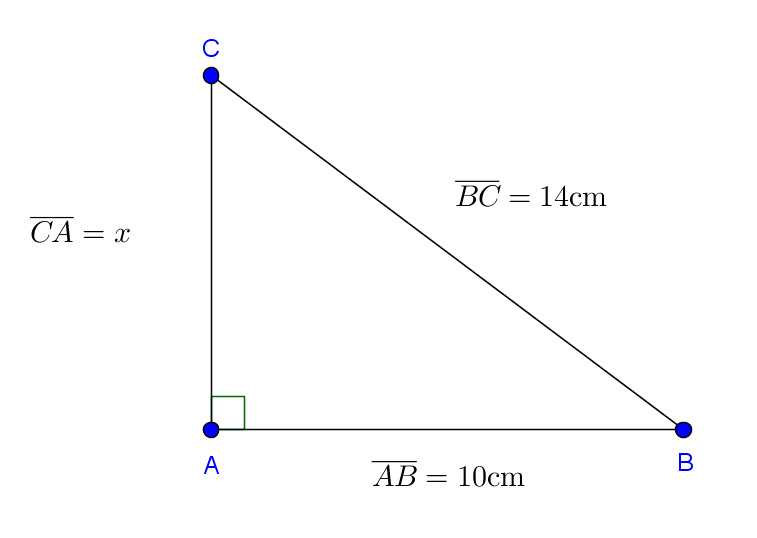
\includegraphics[scale=0.5]{triangulo_retangulo.png}
			\end{tabular} &
			\begin{tabular}{l}
				César Antônio de Magalhães \\
				https://br.linkedin.com/in/cams7
			\end{tabular}
		\end{tabular}
	\end{center}
	\begin{enumerate}
		\item A Tabela \ref{derivadas_basicas} representa as derivadas básicas.
		\begin{table}[htb]
			\centering
			\begin{tabular}{|c|c|}
				\hline
				     Função       &           Derivada            \\ \hline
				  $f(x) = x^n$    &     $f'(x) = nx^{n - 1}$      \\ \hline
				$f(x) = \log_a x$ & $f'(x) = \dfrac{1}{(\ln a)x}$ \\ \hline
			\end{tabular}
			\caption{Tabela básica de derivadas.}
			\label{derivadas_basicas}
		\end{table}
	\end{enumerate}				
\end{document}
